\chapter{Architectuur}\label{ch:Architectuur}

Om inzicht te verkrijgen in potentiële kwetsbaarheden in de projecten van Eaglescience moet er een applicatie worden ontworpen die in staat is om analyses uit te voeren op het moment dat er veranderingen worden aangebracht in deze projecten. Daarnaast moet de applicatie in staat zijn deze analyses uit te voeren op een periodieke basis.
Op het moment van schrijven wordt er binnen Eaglescience ontwikkeld in de talen Scala en NativeScript, maar de verwachting is dat er in de toekomst een mogelijkheid bestaat dat dit uitgebried gaat worden. Daarnaast is zijn deze twee talen niet de enige twee platformen binnen de stack, zo wordt er ook gebruik gemaakt vam docker met daarbnij verschillende images die ook kwetsbaarheden kunnen bevatten. Dit ontwerp voorziet niet in de mogelijkheid om deze toekomstige platformen als ook docker te kunnen scannen. Het ontwerp moet wel zo zijn dat er een mogelijkheid bestaat om deze op een relatief makkelijke manier toe te voegen.

Analyses worden uitgevoerd op modulenniveau, hier zijn in basis twee redenen voor. Ten eerste is een module binnen een Eaglescience project een afgeschermd onderdeel dat een eigen platform benut. Ten tweede kan er op module niveau veranderingen worden verwacht ten opzichte van dependency declaraties.

In figuur~\ref{fig:SOUP-Components} is te zien welke componenten er nodig zijn om van informatie welke middels een Software Composition Tool(SCA) is verkregen te verwerken naar een rapport die in de portal te zien is. De verschillende componenten worden ieder in een eigen sectie uitvoerig besproken. Echter zijn dit de hoofdpunten:
\begin{itemize}
    \item \textbf{Jenkins} Op het moment dat er in Jenkins een build wordt gedaan is er potientieel iets veranderd in de sourcecode en daarmee ook in de dependencies die er beschreven staan in de module. Door de SCA tooling hier al in te zetten kan er direct een rapport worden gegenereert die zichtbaar is in de portal. Hierdoor is er bijna direct inzicht in welke kwetsbaarheden er bekend zijn in het project. In de pipeline moet een onderdeel worden toegevoegd waardoor de SCA tooling kan worden uitgevoerd. Een een BashScript dat een HTTP POST naar de SOUP API kan doen met daarin gegeven over de geanalyseerde module en het project. Eaglescience werkt met Tags om functionaliteiten binnen de pipeline te kunnen sturen het is wenselijk om hier een tag voor de soup analyse toe te voegen om eventueel de analyse uit te schakelen als dit wenselijk is.
    \item \textbf{Portal} De portal is een inhouse applicatie welke gebruikt wordt voor administratieve zaken binnen het bedrijf. de wens is om hier functionaliteiten aan toe te voegen die bedrijfsbreed zijn en daarmee dus project oversteigend zijn. Voor deze applicatie dient er een module te worden toeegevoegd die fungeert als een interface waarin informatie over de bekende kwetsbaarheden te vinden is. maar ook instellingen kunnen worden
    \item \textbf{Analysis Environment} deze omgeving moet het mogelijk maken om vanuit de SOUP API een analyse uit te voeren op modulen. waarbij er een docker container wordt gestart een analyse uitgevoerd wordt en vervolgens de container wordt vernietigd. de voornaamste reden is dat er door de opzet van npm/node en sbt/scala veel combinatie kunnen ontstaan die ervoor kunnen zorgen dat er de versies die gebruikt worden veranderen. Om deze reden moet de analyse omgevingen een nagenoeg exacte kopie zijn van de omgeving op productie.
    \item \textbf{SOUP API} De SOUP API is het centrale deel Het is verantwoordelijk voor het verwerken van de rapporten die door de SCA tools worden opgemaakt. Het is ook verantwoordelijk voor de controle op de analyse omgevingen die het periodiek analyseren mogelijk maken. ALs laatste moet het een API zijn voor de gegevens die op de portal te zien zijn alsook de verwerker van projectsettings.
    \item \textbf{Database} De gekozen database is nu MongoDB LATER MEER WELLICHT WORDT HET NOg MYSQL
\end{itemize}


% OUD
Om bruikbare informatie te kunnen tonen aan de gebruiker moet de informatie dat door de Software Composition Analysis (SCA) Tool wordt geleverd worden bewerkt naar een datamodel waarbij alleen de informatie die relevant is om te tonen wordt opgeslagen. Daarnaast moet het systeem in staat zijn om periodiek een analyse uit te voeren op projecten die bekend zijn binnen de module. In figuur~\ref{fig:SOUP-Components} is te zien hoe onderdelen met elkaar in verbinden staan.
In de secties hieronder wordt ieder onderdeel verder uitgwerkt op een architectonisch niveau.
%OUD


\begin{figure}[bth]
    \myfloatalign
    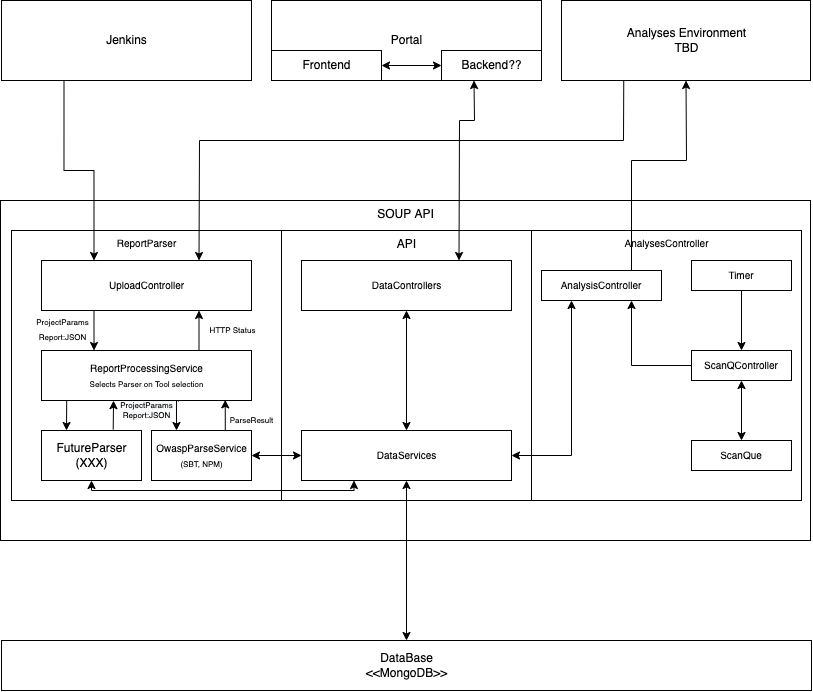
\includegraphics[width=15cm]{gfx/SOUPAPI-SOUPAPI MODULES}
    \caption{Componenten SOUP Analyse Systeem}
    \label{fig:SOUP-Components}
\end{figure}
%    \begin{figure}[bth]
%    \myfloatalign
%    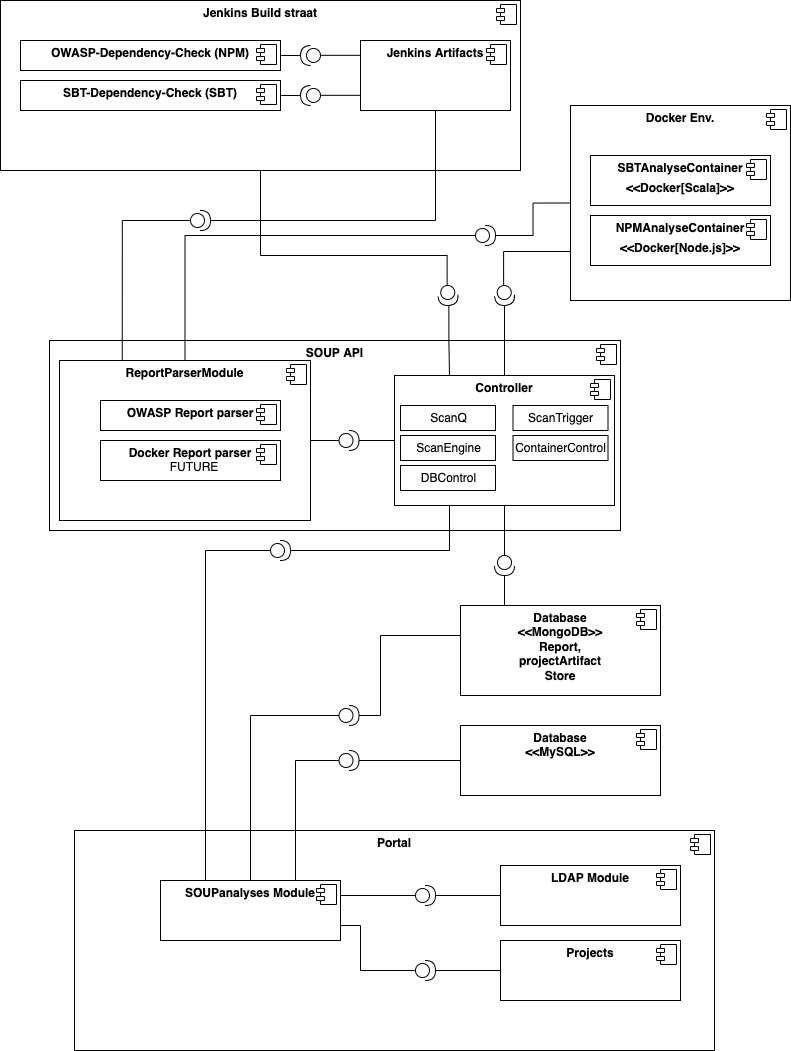
\includegraphics[width=10cm]{gfx/UMLcomponentDiagram}
%    \caption{Componenten SOUP Analyse Systeem}
%    \label{fig:SOUP-Components}
%\end{figure}




\section{SOUPAPI}\label{sec:soupapi}
De SOUP API staat centraal in het nieuwe systeem en is verantwoordelijk voor alle kerntaken die het nieuwe systeem moet uitvoeren. De twee hoofdtaken zijn: "Periodieke scannen van projecten " en "Verwerking van gegevens uit de verkregen resultaten uit de Software Composition Analysis Tool(SCA) en Jenkins, dat gebruikt wordt om een analyse uit te voeren."

\subsection{Intern datamodel}\label{subsec:intern-datamodel}
Het interne datamodel voorziet in de informatie die benodigd is voor medewerkers om beslissing te maken over het handelen met gevonden kwetsbaarheden.
\begin{figure}[bth]
    \myfloatalign
    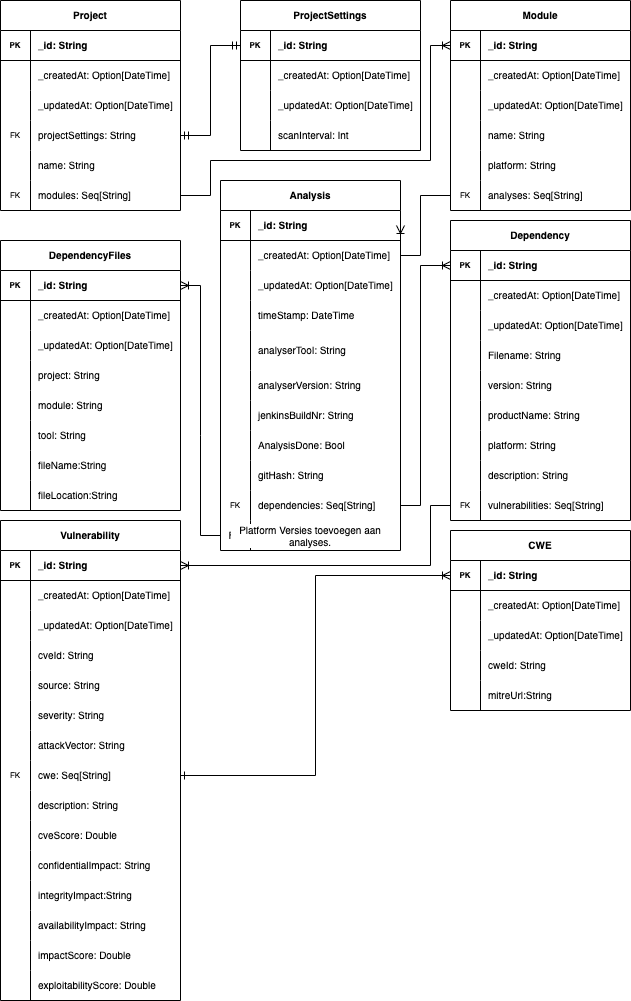
\includegraphics[width=10cm]{gfx/SOUPAPI-SOUPAPI DM}
    \caption{Intern Datamodel}
    \label{fig:SOUP-SoupApiDm}
\end{figure}
%TODO checken of 8pt leesbaar is op print
%TODO tekst beter structureren
In figuur (~\ref{fig:SOUP-SoupApiDm}) is het interne datamodel te vinden waarin de data die opgeslagen dient te worden in afgebeeld. Ook de relaties tussen de verschillende is te zien en worden hieronder verder beschreven.

Een analyses wordt uitgevoerd op een module.

Eaglescience werkt op projectbasis, waarbij één of meer modulen de applicatie vormen. Deze worden dan ook in project opgeslagen naast de naam van het project en projectSettings welke gebruikt worden door de SOUPAPI om te fungeren. Onder projectsettings staat nu een scanInterval die ingesteld kan worden in een aantal dagen dat er tussen de analyses mag zitten. ProjectSettings is bewust apart genomen omdat dit de ruimte bied om de toekomst benodigde instellingen toe tevoegen.

Voor de module wordt de naam en het platform waarin het geschreven is opgeslagen. Aan de de modulen worden de analyses gehangen. Analyses worden gedaan op moduleniveau en niey op projectniveau. Dit geeft de mogelijkheid om de modulen los van elkaar te kunnen analyseren en hier de data van op te slaan.

In de analsyses wordt de timestamp opgeslagen om te achterhalen wanneer deze is uitgevoerd. Als ook het buildnummer uit jenkins als deze is uitgevoerd binnen de jenkins timeline. Ook wordt de githash opgeslagen om op die manier te kunnen achterhalen welke commit er geanalyseerd is.

De analyses bevat een lijst met dependencies die in de modules voorkomen. Voor deze dependencies worden de filenaam, versie, productnaam, en platform opgeslagen. Als ook een descriptie als deze wordt meegegeven door de SCA Tool. Als de dependency een Vulnerability beavt wordt deze aan de dependency toegevoegd. de Vulnerability bevat impactscores voor confidentiality, integrity en availability als een algehele impact score. Ook wordt de CWE opgeslagen waarin het id en de url naar meer informatie wordt opgeslagen.

Op het moment dat een analyse is uitgevoerd in de Jenkins pipeline worden ook de files waarin de dependency declaraties staan op geslagen per Analyse. Deze dependency files kunnen op een later moment worden gebruikt om een analyse uit te voeren voor een project of module.

\subsection{Verwerking gegevens vanuit de builds}\label{subsec:verwerking-gegevens-vanuit-de-sca}
De belangrijkste taak van de SOUP API is het verwerken van de gegevens die bechikbaar worden gemaakt vanuit een analyse door de SCA Tooling. De gegevens komen binnen van twee verschillende processen:
\begin{itemize}
    \item Jenkins buildstraat
    \item Intern periodiek scan systeem (nog betere naam vinden)
\end{itemize}
In figuur(~\ref{fig:UploadReportFlow}) is te zien hoe een upload van een raport wordt verwerkt. Er is gekozen om twee endpoints aan te bieden voor de twee verschillende processen die verantwoordelijk zijn voor het aanleveren van een rapport. Eén endpoint waar het process binnen Jenkins het rapport.json en dependency declaraties kan verstuen en Eén endpoint waar het periodieke systeem het rapport kan versturen.
Beide endpoints bevatten Parameters om extra meta data mee te sturen die informatie bevatten over welkeproject/module het gaat. En in het geval van de jenkins endpoint ook de Githash waar jenkins de build voor heeft gedaan en het resulterende jenkinsBuildnummer. De laatst parameter die meegestuurd wordt is de selector voor de gebruikte tool waarmee de reportService de juiste parser kan kiezen.

Dit ontwerp is voorzien van een OWASPReportParser welke gebruikt kan worden om de rapporten gegenereerd door de OWASP tool om te zetten naar het interne datamodel. Door gebruik te maken van een tussenliggende service is het mogelijk om hier meerdere parsers aan toe te voegen zodat in de toekomst andere parsers geschreven kunnen worden die een rapport van een toekomstige tool om kan zetten in hetzelfde interne datamodel.


\begin{figure}[bth]
    \myfloatalign
    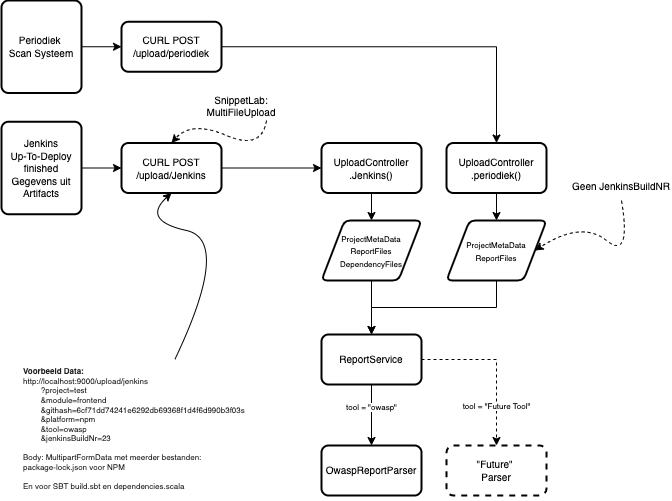
\includegraphics[width=10cm]{gfx/SOUPAPI-UploadAnalysis}
    \caption{Upload Report Flow}
    \label{fig:UploadReportFlow}
\end{figure}

Zoals eerder benoemd is de OWASP parser verantwoordelijk voor het inlezen van een aangeboden JSON en deze vervolgens op te slaan in een database op basis van het interne datamodel. Om dit te bewerkstelligen dienen de volgende stappen te worden genomen:
Als eerst wordt er gekeken of het in de parameters meegegeven project bestaat binnen de SOUPAPI. Als dit het geval is dan wordt er gekeken of de meegegeven module in het project bestaat. Mocht het project niet bestaan dan wordt er één aangemaakt samen met de meegegeven module en de default SOAPAPI projectsettings. Mocht de module niet bestaan dan wordt deze aangemaakt met de parameters die meegegeven zijn en vervolgens toegevoegd aan het project.
Op het moment dat zowel het project als de module bestaan wordt er een analyse aangemaakt en toegevoegd aan de
module. Als het een upload is vanuit het JenkinsProces worden de meegezonden dependency declaraties opgeslagen. Daarnaast wordt er voor iedere dependency in het rapport bekeken of deze al in de database staat. Als dit het geval is dan wordt deze toegevoegd aan de analyse. Als de dependency nog niet bestaat wordt deze opgeslagen in de database en vervolgens toegevoegd aan de analyse. Vervolgens wordt de vulnerability toegevoegd en gelinkt aan de dependencies. en ook hier geld als de vulnerability al bestaat is er alleen een link nodig.
Als laatst wordt er een nieuwe analyse toegevoegd aan de scanQ waarna er een result HTTP 200/201 komt.
\begin{figure}[bth]
    \myfloatalign
    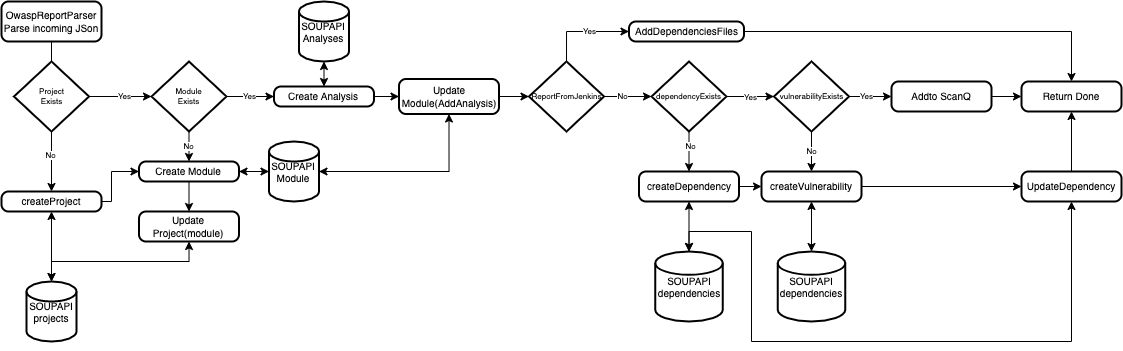
\includegraphics[width=15cm]{gfx/SOUPAPI-ReportParseFlow}
    \caption{Owasp Report Flow}
    \label{fig:OwaspReportFlow}
\end{figure}

\subsection{AnalysesController}\label{subsec:controller}
Naast de analyses die van de rapporten die uit het jenkins process komen is er ook behoefte om periodiek te analyseren op oudere niet actieve projecten. Om dit te kunnen faciliteren omnvat de Analyses controller een aantal componenten die ieders verantwoordelijk zijn voor een eigen taak:

\begin{figure}[bth]
    \myfloatalign
    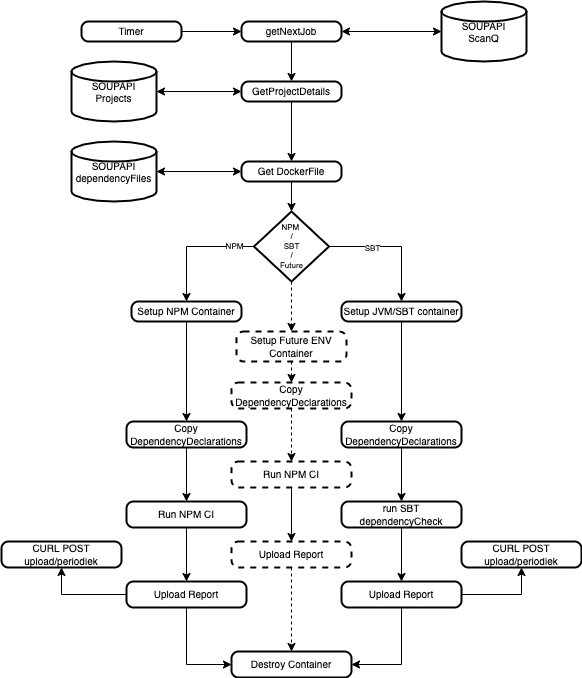
\includegraphics[width=10cm]{gfx/SOUPAPI-Periodic Analysis}
    \caption{Periodieke analyse flow}
    \label{fig:PeriodicAnalysis}
\end{figure}

\subsubsection{Timer}
De timer is verantwoordelijk voor het op tijd starten van de periodieke analyses op projecten die in de ScanQ staan. Op het moment dat er een geplannde analyse uitgevoerd moet worden zal deze aan de analyses controller worden gegeven die de verantwoordelijkheid overneemt.
\subsubsection{ScanQ + ScanQController}
De scanQ is een datastructuur gebasseerd op een list/seq waarin de analyses opgeslagen zijn die uitgevoerd moeten worden. De ScanQcontroller regelt de mutaties op deze scanQ.
\subsubsection{AnalysesController}
De analyse controller dient de taken uit te voeren die in figuur(~\ref{fig:PeriodicAnalysis}) weergegeven zijn. Dit is een sequenteel proces waarbij de controller wacht op antwoord voordat het een volgend onderdeel begint.



De rapporten uit het JenkinsProces vormen de basis van de analyse. Op het moment dat een analyse is toegevoegd worden ook de dependency declaraties opgeslagen. Deze declaraties vormen de basis voor de period

\subsection{API}\label{subsec:api}


\section{Jenkins buildtstraat}\label{sec:jenkins-buildtstraat}
Op het moment dat er een project wordt gebouwd middels de Jenkins buildstraat kan er vanuit worden gegaan dat er wijzigingen zijn in de sourcecode. Mogelijk zijn er dan ook wijzigingen in de declaraties in bijvoorbeeld versies en of nieuwe of andere dependencies de gebruikt worden. In het nieuwe systeem wordt Jenkins gebruikt om deze informatie in het systeem te verkrijgen. Om deze informatie in de SOUP API te krijgen moeten er een aantal aanpassingen gedaan worden die ervoor zorgen dat informatie omtrend kwetsbaarhden in een uniforme manier worden gewonnen en verstuurd naar de SOUP API.

\subsection{Data}\label{subsec:jenkins_Datamodel}
De informatie die uit Jenkins wordt verkregen is informatie waarop op een later moment de periodieke analyses worden gebaseerd. De data die verstuurt wordt moet dan ook het volgende bevatten: Data over de identiteit van het project en welke modulen er aanwezig zijn. De rapporten die gegenereerd zijn door de in de pipeline aanwezige analyse tools. En de dependencies die gebruikt worden. Om de data in een zo universeel mogelijke manier te versturen wordt het data transfer model genbruitk die in listing~\ref{lst:DTMJenkins} te zien is. Het model bestaat uit drie hoofddelen waarin de gegevens over de analyse en het project zijn opgeslagen, De Rapporten die gegenereerd worden door de SCA tooling ingebouwd in de pipeline waarbij ook de tool is meegegeven. En van iedere module een lijst met dependencies.
\begin{lstlisting}[caption={Data transfer model vanuit Jenkins},label=lst:DTMJenkins]
{
  "projectnaam": "GroeiGids",
  "BuildHash": "fb5f5cb47bbd0cbf2f4771c55242fedbf41c5efc",
  "buildDate": "22-01-2022",
  "buildModules": [
    "App",
    "portal",
    "backend"
  ],
  "reports": [
    {
      "NPM-portal-report": {
        "tool": "OWASP-NPM",
        "report": {}
      }
    },
    {
      "NPM-app-Report": {
        "tool": "OWASP-NPM",
        "report": {}
      }
    },
    {
      "sbt-backend-report": {
        "tool": "OWASP-SBT",
        "report": {}
      }
    }
  ],
  "dependencies": [
    {
      "npm-portal-deps": {
        "dependencies": [
          {
            "naam": "<<NAAM>>",
            "versie": "<<Versie>>"
          }
        ],
        "devDependencies": [
          {
            "naam": "<<NAAM>>",
            "versie": "<<Versie>>"
          }
        ]
      }
    },
    {
      "npm-app-deps": {
        "dependencies": [
          {
            "naam": "<<NAAM>>",
            "versie": "<<Versie>>"
          }
        ],
        "devDependencies": [
          {
            "naam": "<<NAAM>>",
            "versie": "<<Versie>>"
          }
        ]
      }
    },
    {
      "sbt-backend-deps": {
        "dependencies": [
          {
            "naam": "<<NAAM>>",
            "versie": "<<Versie>>"
          }
        ]
      }
    }
  ]
}
\end{lstlisting}

\subsection{informatie extractie methoden en verzending van de informatie}

Voor iedere module in een project moet de betreffende SCA tool worden aangeroepen waatbij het Rapport wordt toegevoegd aan de Jenkins Artifacts.
Op het moment dat de deploy gedaan is moeten deze rapporten samen worden gevoegd met de metadata tot een JSON bestand welke vervolgens middels een POST methode kan worden vertuurt naar de SOUP API welke het vervolgen middels de Parser toevoegd aan de database en scheduler als zijn een bestaand project die periodiek moet worden geanalyseerd.


\section{Portal}\label{sec:portal}
In de portal wordt er een module toegevoegd die als interface dient voor het SOUP-analyse systeem. Informatie over kwetsbaarheden in geanalyseerde projecten worden hier weergegeven. Ook is het hier mogelijk om per project in te kunnen zien welke instellingen er gelden voor analyses en waar zo nodig kunnen deze hier worden aangepast.
In de module moet er dus een plek komen waar informatie betreft kwetsbaarheden kan worden geraadpleegd. Daarnaast moet en er een plek komen waarbij instellingen kunnen worden aangepast zodat de analyses worden uitgevoerd op de ingesteld periode. En of aan en uit gezet kan worden.

In de komende hoofdstukken zullen de dir ehoofd modulen verder worden uitgwerkt in een functioneel ontwerp
